\chapter{Introducción General}

\label{Chapter1}

El capítulo presenta los temas principales abordados en el trabajo con la
intención de orientar al lector en las estrategias de desarrollo
implementadas.

\section{SDI en la Industria de la Televisión}

En el ámbito televisivo, es frecuente la necesidad de transmitir señales
digitales no comprimidas a través de medios compatibles con los formatos
analógicos. Con este propósito, numerosos dispositivos de televisión digital,
tales como codificadores H.264, distribuidores y matrices digitales, están
equipados con interfaces digitales serie conocidas como SDI (del inglés
\textit{Serial Digital Interface}). El estándar SDI constituye una interfaz
digital serie asincrónica diseñada principalmente para la transmisión de señales
de video digital no comprimido y sin encriptar.

Esta tecnología de transmisión se implementa comúnmente mediante un único
conductor, generalmente cables coaxiales de 75 Ohms, que son el estándar para
la televisión. Fue concebida para transmitir video digital en un entorno
compatible con el video analógico y se utiliza también para la transmisión de
paquetes de datos o audio. Una característica destacada de este estándar es su
capacidad para admitir tasas de bits muy elevadas y presentar bajos retardos de
propagación, lo que lo convierte en una elección común en aplicaciones donde se
requiere la transmisión de video de alta calidad. Debido a la elevada tasa de
datos, su implementación suele limitarse a distancias cortas, siendo su uso más
común en entornos profesionales.

En la actualidad, la visualización de video es indispensable no solo en los
sistemas de transmisión de televisión, sino también en diversos dispositivos de
monitoreo. La tecnología temprana de televisión digital se centraba
principalmente en el sistema de estudio. A medida que la tecnología de
televisión digital maduraba, especialmente durante la transición de CATV de un
sistema analógico a uno digital, tanto la tecnología como los dispositivos de
televisión digital se han vuelto ampliamente utilizados en los sistemas de
transmisión. Para adaptarse a diferentes entornos de aplicación, han surgido
diversas interfaces de televisión digital, como ASI en DVB, ISBD-Tb, SSI y SPI,
entre otras.

\section{Introducción a Interfaz Digital Serie (SDI)}

La Interfaz SDI es una familia de interfaces de video digital estandarizada por
por SMPTE (Society of Motion Picture and Television Engineers en inglés) en
1989. Se trata de un estándar para la transmisión de video y audio digital sin
comprimir mediante cables coaxiales o más recientemente de fibra óptica.

Su aplicación abarca diferentes niveles de resolución, desde definición
estándar (SD) hasta resoluciones de alta definición (HD) y ultra alta
definición (UHD), lo que la convierte en una opción versátil para diversas
aplicaciones en la producción y transmisión de contenido audiovisual.

Además, las interfaces SDI son altamente versátiles y admiten una variedad de
resoluciones, desde definición estándar hasta ultra alta definición, adaptándose
así a las crecientes demandas de la industria en términos de calidad de imagen.
Su capacidad para transmitir señales de video de manera confiable y eficiente
las hace óptimas para una amplia gama de equipos, incluyendo cámaras de video,
monitores, mezcladores de video, unidades de grabación, servidores de video, y
sistemas de transmisión en vivo. En el contexto de la producción y
postproducción audiovisual, las interfaces SDI se integran de manera crucial en
equipos como grabadores digitales, sistemas de edición no lineal (NLE) y 
matrices de conmutación, proporcionando una conectividad robusta y sin pérdida
para garantizar la calidad del flujo de trabajo audiovisual.

\section{Estado del Arte}

A lo largo del tiempo, la SDI ha evolucionado con diferentes estándares. Estos
estándares incluyen variantes como SD-SDI, HD-SDI, 3G-SDI, sobre las que se
hará foco en este trabajo y versiones de mayor velocidad como 6G-SDI, 12G-SDI
y 24G-SDI, cada uno diseñado para satisfacer las demandas crecientes de calidad
y resolución en la industria.

La Tabla~\ref{tab:sdi_standards} muestra la evolución de los estándares a lo largo del tiempo:

\begin{table}[h]
    \centering
    \begin{tabular}{cccccc}
        \toprule
        \textbf{Standard} & \textbf{Nombre} & \textbf{Fecha} & \textbf{Bitrates} & \textbf{Ejemplos de aplicación} \\
        \midrule
        SMPTE 259M      & SD-SDI    & 1989 & 360 Mbit/s     & 480i, 576i \\
        SMPTE 344M      & ED-SDI    & 2000 & 540 Mbit/s     & 480p, 576p \\
        SMPTE 292M      & HD-SDI    & 1998 & 1.485 Gbit/s   & 720p, 1080i \\
        SMPTE 372M      & Dual Link & 2002 & 2.970 Gbit/s   & 1080p60 \\
        SMPTE 424M      & 3G-SDI    & 2006 & 2.970 Gbit/s   & 1080p60 \\
        SMPTE ST-2081   & 6G-SDI    & 2015 & 6 Gbit/s       & 2160p30 \\
        SMPTE ST-2082   & 12G-SDI   & 2015 & 12 Gbit/s      & 2160p60 \\
        SMPTE ST-2083   & 24G-SDI   & 2020 & 24 Gbit/s      & 2160p/4k@120, 8k@60 \\
        \bottomrule
    \end{tabular}
    \caption{SDI Standards and Characteristics}
    \label{tab:sdi_standards}
\end{table}

Las interfaces SDI se han convertido en la columna vertebral de la industria
audiovisual debido a su confiabilidad y capacidad para transmitir señales de
video y audio digital sin comprimir. Su uso generalizado se debe a varias
razones fundamentales. En primer lugar, las interfaces SDI garantizan la
transmisión de señales de alta calidad, preservando la integridad de la
información digital y evitando la pérdida de calidad que podría ocurrir con la
compresión. Esto es especialmente crucial en entornos profesionales donde la
fidelidad de la imagen y el sonido es primordial.

\section{Implementación de SDI en FPGA}

Una FPGA (del inglés \textit{Field-Programmable Gate Array}) se presenta como
una elección ideal para el desarrollo de una interfaz SDI por varias razones
fundamentales. En primer lugar, la naturaleza configurable y programable de las
FPGA permite adaptar su lógica interna para cumplir con los requisitos
específicos de la interfaz SDI. Dado que los estándares SDI pueden abarcar
diversas resoluciones, tasas de bits y formatos, la flexibilidad inherente de
las FPGA facilita la implementación de estas variaciones sin necesidad de
cambiar el \textit{hardware}. Esto resulta esencial en un entorno tecnológico
en constante evolución, como el de la transmisión de video.

Además, las FPGA ofrecen un alto rendimiento y paralelismo, lo que resulta
crucial en el procesamiento de datos en tiempo real requerido por las interfaces
SDI. La capacidad de realizar múltiples tareas de manera simultánea y gestionar
grandes volúmenes de datos a alta velocidad hace que las FPGA sean aptas para
manejar los flujos de información complejos y exigentes de las señales de video
y audio sin comprimir.

\section{Motivación}

\vspace{1cm}
\begin{figure}[htbp]
    \centering
    \begin{minipage}{.45\linewidth}
        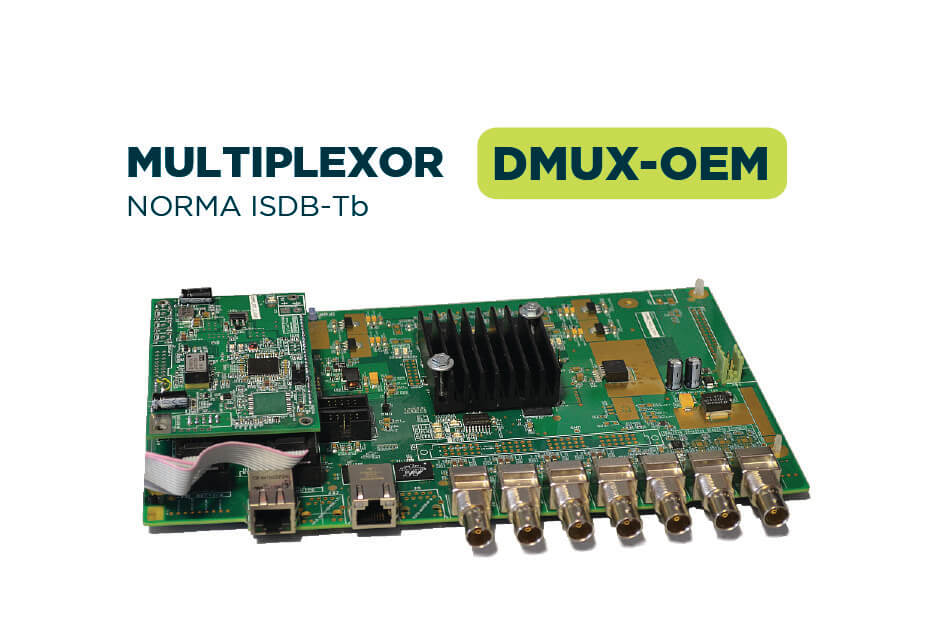
\includegraphics[width=\linewidth]{./Figures/DMUX-OEM.jpg}
        % \caption{First caption}
        % \label{fig:vs-mux}
    \end{minipage}
    \hspace{.05\linewidth}
    \begin{minipage}{.45\linewidth}
        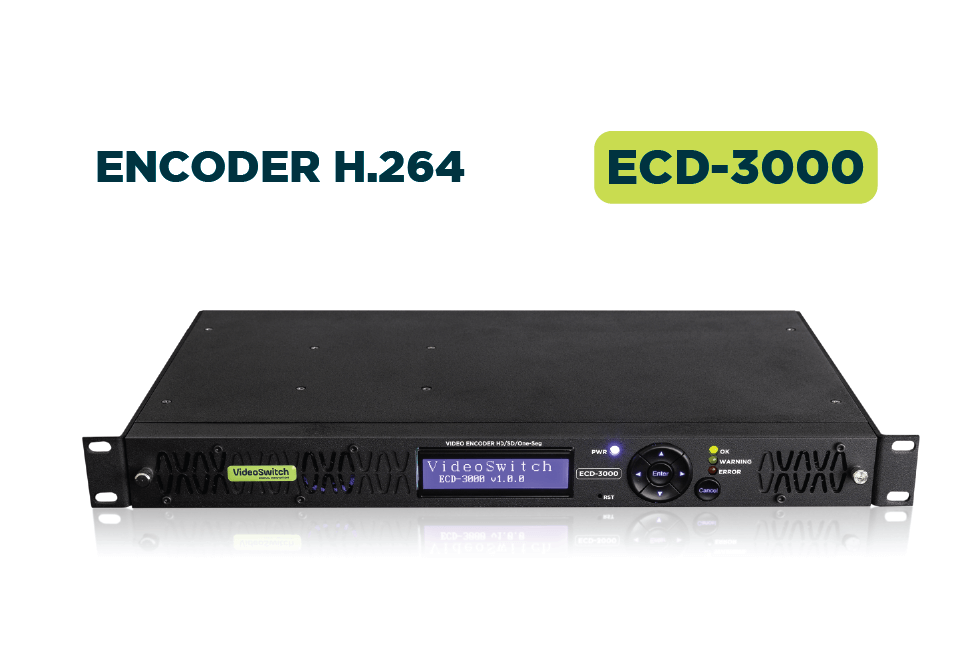
\includegraphics[width=\linewidth]{./Figures/ECD-3000.png}
        % \caption{Second caption}
        % \label{fig:vs-ecd}
    \end{minipage}
    \caption{Productos VideoSwitch, Izquierda: Multiplexor Digital - Derecha: Encoder H.264}
        \label{fig:vs-mux-ecd}
\end{figure}
\vspace{1cm}

VideoSwitch SRL \citep{vs-srl} es la empresa líder en Argentina y Hispanoamérica
en el desarrollo de equipos, soluciones y servicios para la transmisión y
acondicionamiento de video en la industria de la televisión, como por ejemplo
Multiplexor ISBD-Tb o un \textit{Encoder} H.264, Figura~\ref{fig:vs-mux-ecd},
dos productos de la marca en los que se podría implementar la solución propuesta.
Al plantear este trabajo, la empresa se encontraba vinculada a un único
fabricante de FPGAs y a una versión específica de su \textit{software} de
diseño debido a la dependencia de varios productos con un módulo propietario o
IP (del inglés \textit{Intellectual Property}) que implementaba la interfaz SDI
de la empresa proveedora. Esto implicaba la imposibilidad de aprovechar las
ventajas de programas más modernos o de otras empresas, así como la dependencia
de una sola marca de dispositivos programables. En situaciones de crisis de
disponibilidad de semiconductores, como la ocurrida durante la pandemia, se
evidencia la necesidad de que las empresas puedan independizar su producción de
un único proveedor. Por todas estas razones, el desarrollo propuesto se vuelve
estratégico para una empresa de esta envergadura.
